% embodimetry --- ~11-page arXiv writeup (cs.RO primary, cs.LG secondary).
% Capability-Ladder Audit framing: L0 pretrained / L1 fine-tune / L2 classical
% / L3 world-model planner on ONE seed+Wilson-CI+MDE contract. The LEAD
% contribution is the auditable instrument + the self-caught normalization
% bug (ACT x aloha 0.016 -> 0.824 via a clean 2x2 ablation) + the v1.1
% suite-averaged SmolVLA/LIBERO protocol-gap audit. L3 is a
% STRENGTHENED-BUT-QUALIFIED result: under matched RECEDING-HORIZON MPC,
% zero-training world-model latent-MPC planning reaches 4/6 (JEPA-WM) ~
% 3/6 (DINO-WM) on Wall NAVIGATION while CONTACT (PushT) yields zero
% successes in both families (JEPA-WM 0/6, DINO-WM 0/2 -- the DINO-WM
% PushT run stopped at 2 episodes inside its GPU box), and the
% nav-not-contact direction REPLICATES across the two WM families (DINO-WM,
% facebookresearch/jepa-wms). The earlier one-shot 0/6 JEPA-WM Wall was a
% PLANNING-PROTOCOL artifact, corrected by a protocol control. CAVEATS kept
% in text: N<=6 per cell (small; no per-family contrast significant), ONE
% env per endpoint (two-endpoint contrast, NOT a curve / cross-env law);
% gradient MIDDLE unmeasured (MetaWorld anchor = future work). L3 numbers
% are a CROSS-REPO artifact (lerobot-wm-research, private: available on
% request, release planned), cited as such.

\documentclass[10pt]{article}

\usepackage[a4paper,top=0.7in,bottom=0.7in,left=0.75in,right=0.75in]{geometry}
\usepackage[utf8]{inputenc}
\usepackage[T1]{fontenc}
\usepackage{lmodern}
\usepackage{microtype}
\usepackage{amsmath,amssymb}
\usepackage{booktabs}
\usepackage{multirow}
\usepackage{subcaption}
\usepackage{graphicx}
\usepackage{xcolor}
\usepackage{hyperref}
\usepackage{url}
\usepackage{multicol}
\usepackage[compact]{titlesec}
\titlespacing*{\section}{0pt}{1.1ex plus 0.3ex minus 0.2ex}{0.6ex plus 0.2ex}
\titlespacing*{\subsection}{0pt}{0.8ex plus 0.2ex minus 0.2ex}{0.4ex plus 0.1ex}
\titlespacing*{\paragraph}{0pt}{0.6ex plus 0.2ex minus 0.1ex}{1em}

% Relax LaTeX's default float-placement fractions -- with 4 tables + 3
% figures in a 10pt two-column-tight single-column doc, the defaults
% (topfraction 0.7, textfraction 0.2, 2 floats/page) queue every float past
% the text that references it and dump them on their own near-empty trailing
% pages. This lets floats interleave with text instead.
\renewcommand{\topfraction}{0.9}
\renewcommand{\bottomfraction}{0.8}
\renewcommand{\textfraction}{0.07}
\renewcommand{\floatpagefraction}{0.75}
\setcounter{topnumber}{4}
\setcounter{bottomnumber}{2}
\setcounter{totalnumber}{6}

\hypersetup{
    colorlinks=true,
    linkcolor=blue!50!black,
    citecolor=blue!50!black,
    urlcolor=blue!50!black,
}

% \todo marks a number not yet pinned to an in-tree parquet/JSON value.
% Render it visibly so a human resolves it before submission.
\newcommand{\todo}[1]{\textcolor{red}{[\textbf{TODO:} #1]}}

\title{\vspace{-1.5ex}embodimetry: a Capability-Ladder Audit ---
one self-auditing eval contract for pretrained, fine-tuned, classical,
and world-model-planner robot policies\vspace{-0.5ex}}
\author{Th\'eo Hermann\\
\texttt{thermann.ai@gmail.com} \quad
\texttt{https://github.com/thrmnn/embodimetry}}
\date{\vspace{-2ex}\today\vspace{-1ex}}

\begin{document}

\maketitle

% ---------------------------------------------------------------- %
% Abstract                                                         %
% ---------------------------------------------------------------- %

\begin{abstract}
Robot-policy success rates are reported per paradigm --- pretrained
imitation, fine-tuning, classical control, world-model planning --- on
incompatible protocols, so the paradigms cannot be put on one axis. We
introduce \emph{embodimetry}, a \emph{Capability-Ladder Audit} that scores
all four paradigms as the \emph{same} \texttt{PolicyCallable} under one
seed / confidence-interval / minimum-detectable-effect contract on shared
LeRobot~\cite{cadene2024lerobot} tasks, with floor baselines and honest
negatives kept on the board. The instrument audits itself: it caught a
normalization bug in \emph{our own} harness that pinned ACT at $0.016$
(below the env's random floor); a controlled $2{\times}2$ ablation
attributed the $0.016\to0.824$ recovery to the fix, and a guard test
code-enforces that every result keeps its caveats. Pointed outward, the
contract measures a protocol-level discrepancy against SmolVLA's published
LIBERO suite averages in all four suites ($-10.7$ to $-27.6$\,pp;
task-as-sampling-unit $t$-tests, Holm-adjusted $p\le0.037$; the goal gap
is smallest and statistically
marginal). At the top rung, under matched receding-horizon MPC, a
zero-training world-model planner reaches $4/6$ (JEPA-WM) and $3/6$
(DINO-WM) on Wall navigation but zero successes on PushT contact ($0/6$
and $0/2$), a direction not specific to one world-model
family --- a two-endpoint contrast at $N{\le}6$ episodes per cell, not a
cross-env law.
\end{abstract}

% ---------------------------------------------------------------- %
% Introduction                                                     %
% ---------------------------------------------------------------- %

\section{Introduction}

Robot control is pursued along a ladder of paradigms: \textbf{L0}
zero-shot evaluation of a
pretrained policy, \textbf{L1} fine-tuning it on a small demo
budget, \textbf{L2} hand-engineered classical control, and \textbf{L3}
planning through a learned world model. Each rung reports success its own
way --- a Diffusion Policy
number~\cite{chi2023diffusion}, an ACT fine-tuning
number~\cite{zhao2023learning}, a scripted-controller baseline, and a
world-model planner~\cite{zhou2024dinowm,assran2025vjepa2} are never
measured on a common axis; protocols differ in seed counts, episode
budgets, success thresholds, and whether confidence intervals are reported
at all, a reproducibility gap documented repeatedly in adjacent
fields~\cite{henderson2018deep,agarwal2021deep,patterson2024empirical}.
\textbf{Building a ruler
that scores them together is the load-bearing contribution of this
paper.} We introduce \emph{embodimetry}, a \emph{Capability-Ladder Audit}:
it measures multiple paradigms as the \emph{same} \texttt{PolicyCallable}
(\texttt{obs} $\to$ \texttt{action}) through \emph{one} seed / Wilson-CI /
MDE contract on shared LeRobot~\cite{cadene2024lerobot} tasks, with floor
baselines and honest negatives (the SmolVLA-LoRA collapse, the classical
$0.012$) kept on the board. Neighboring efforts (HF leaderboards, MLPerf,
Open X-Embodiment~\cite{bohg2024open}, the world-model
benchmarks~\cite{zhou2024dinowm,assran2025vjepa2}, and the emerging
evaluation-audit thread of \S\ref{sec:related}) each cover part of this;
to our knowledge, none combines one cross-paradigm ruler with retained
negatives and a \emph{code-enforced self-audit} of its own harness. The
instrument is paradigm-neutral by
construction: it has no stake in which rung wins.

We stand behind three reproducible contributions, developed in
\S\ref{sec:methods}--\S\ref{sec:l3}: \emph{(1)} the single cross-paradigm
contract above; \emph{(2)} a self-auditing methodology, code-fenced against
re-inflation by a guard test (\S\ref{sec:guard}); and \emph{(3)} a
strengthened-but-qualified L3 reading the contract was built to
test --- under matched receding-horizon MPC, zero-training world-model
planning reaches Wall \emph{navigation} but zero PushT \emph{contact}
successes in two independent world-model families, a \emph{two-endpoint}
contrast (\S\ref{sec:l3}) rather than a measured curve or cross-env law.
embodimetry v1 releases open data (a Hugging Face
Hub~\cite{huggingfacehub2024} dataset of every per-episode outcome plus an
MP4 of every rollout, published with v1), open eval (this repository's
pinned pipeline; any parquet row re-derives via
\texttt{scripts/run\_one.py}), and open analysis
(\texttt{src/embodimetry/figures.py} renders every figure here via
\texttt{make paper-figures}). The v1 leaderboard crosses four learned
policies and two weights-free floor baselines with six envs
(22~runnable cells after the checkpoint-availability filter); the ladder
rungs (L1, L2) run as separate
audit cells on the identical contract, gated out of the leaderboard.

The contract's flagship demonstration is that it audits, first, its own
harness: ACT on
\texttt{aloha\_transfer\_cube} read $\hat{p}{=}0.016$, below the env's
random floor, until we traced it to un-normalized image observations; a
clean $2{\times}2$ ablation attributes the $0.016\to0.824$ recovery to the
normalization fix, with the inference-settings effect inconclusive
(\S\ref{sec:results-audit}). A loss curve would never have surfaced this;
only a closed-loop success rate with a confidence interval did --- the
value of a neutral contract is
that it bites on the surface it is supposed to protect, including the
auditor's own. Pointed outward, the same machinery yields the
suite-level protocol finding of \S\ref{sec:suite-audit}. The L0--L2 rungs
are a spine of honest negatives that make the contract trustworthy
(\S\ref{sec:results}), and at the top of the ladder the contract
delivers the two-endpoint world-model study it was built for
(\S\ref{sec:l3}). The benchmark
itself is the data; this paper is the defense.

% ---------------------------------------------------------------- %
% Related Work                                                     %
% ---------------------------------------------------------------- %

\section{Related work}
\label{sec:related}

\paragraph{Robot-learning benchmarks and statistical rigor.}
PushT~\cite{chi2023diffusion}, the Aloha suite~\cite{zhao2023learning},
and LIBERO~\cite{liu2023libero} are the de facto LeRobot references;
RLBench~\cite{james2020rlbench}, CALVIN~\cite{mees2022calvin}, and Open
X-Embodiment~\cite{bohg2024open} offer larger taxonomies but no
pretrained LeRobot-compatible checkpoints or shared protocol. None ship a
multi-policy leaderboard with shared seed accounting, multi-seed CIs, and
re-runnable rows. We adopt the multi-seed, bootstrap-CI, MDE-bounded
posture that Henderson et al.~\cite{henderson2018deep}, Agarwal et
al.~\cite{agarwal2021deep}, and Patterson et
al.~\cite{patterson2024empirical} established for deep RL, and add
weights-free
no-op/uniform-random floor baselines on every cell (per the
Gym~\cite{brockman2016openai} convention) since some envs admit non-zero
random success.

\paragraph{Evaluation rigor and benchmark auditing.}
A growing thread treats robot-policy evaluation itself as the object of
study: best-practice guidance for policy
evaluation~\cite{kressgazit2024robot}, statistical frameworks for
trustworthy performance claims at small
$n$~\cite{vincent2024generalizable}, and simulation-based evaluation
validated against real-robot outcomes~\cite{li2024simpler}. Closest to
our outward-facing audit, vla-eval~\cite{choi2026vlaeval} reproduces
published VLA scores across simulation benchmarks --- including LIBERO,
the canonical open-VLA eval target since
OpenVLA~\cite{kim2024openvla} --- and documents previously undocumented
protocol pitfalls in doing so; LIBERO-Plus~\cite{fei2025liberoplus} and
LIBERO-PRO~\cite{zhou2025liberopro} stress-test LIBERO-evaluated VLAs for
robustness and memorization, complementing our suite-level protocol
finding (\S\ref{sec:suite-audit}). These efforts audit \emph{policies} or
\emph{other} benchmarks; to our knowledge, none makes auditing its
\emph{own} harness a first-class, code-enforced contribution --- a
regression-guarded self-audit (\S\ref{sec:guard}) with a controlled
attribution ablation --- which is the narrower uniqueness claim this
paper defends.

\paragraph{Cross-paradigm and world-model planning.}
The ladder we audit spans paradigms each benchmarked in isolation:
classical control and learned policies are compared only informally, and
world-model planners --- PlaNet~\cite{hafner2019planet},
DINO-WM~\cite{zhou2024dinowm}, V-JEPA-2-AC~\cite{assran2025vjepa2} ---
report success on their own tasks, never against a learned imitation
policy under one shared seed/CI protocol. Our contribution is not a new
policy class but the \emph{contract} that puts a pretrained, fine-tuned,
classical, \emph{and} world-model planner on the same Wilson interval ---
with floor baselines and honest negatives retained, a combination we have
not found in any neighboring benchmark --- plus the \emph{cross-env,
cross-family study it makes
possible}: running the same receding-horizon latent-MPC loop across two
world-model families (DINO-WM, \texttt{jepa-wms}) on envs of differing
dynamical complexity, which yields a two-endpoint reading --- zero-training
planning reaches navigation but records zero contact successes, in both
families (\S\ref{sec:l3}, with its caveats).

% ---------------------------------------------------------------- %
% Methods                                                          %
% ---------------------------------------------------------------- %

\section{Methods}
\label{sec:methods}

\paragraph{Sweep contract.}
The unit of evaluation is a \textit{cell}:
$(\text{policy}, \text{env}, \text{seed\_idx})$ with
$\text{seed\_idx} \in \{0,\ldots,4\}$. Each cell runs $n_\text{ep}$
episodes; the contract is $n_\text{ep}{=}50$ unless the auto-downscope
rule (below) reduces it, giving $N = 5 \cdot 50 = 250$ binary outcomes.
An episode runs from \texttt{env.reset(seed=$s$)} until
\texttt{terminated}, \texttt{truncated}, or step count reaches
env-specific \texttt{max\_steps} (PushT 300, Aloha 400, LIBERO
$\{280,280,300,520\}$ for spatial/object/goal/10, inherited from
lerobot defaults; canonical LIBERO uses 600 for all four, an audit
caveat in Section~\ref{sec:results-audit}). Success is the per-env
\texttt{SUCCESS\_REWARD} threshold; the episode succeeds iff its
final-step reward meets or exceeds it. PR~\#90 adds a selectable
\texttt{--canonical} criterion (paper termination rule, 600-step LIBERO
cap); v1 ships the \texttt{v1\_legacy} (final-reward-threshold)
criterion --- not lerobot's canonical sticky-success reduction; lerobot
defaults supplied only the step caps. (\emph{Sticky} semantics, used by
the ladder cells: an episode succeeds if the condition held at \emph{any}
step --- \texttt{sticky\_is\_success} reduces \texttt{any(is\_success)},
\texttt{sticky\_reward\_eq} reduces
\texttt{any(reward\,${=}$\,threshold)}; each table states the criterion
its cells ran.) The v1.1 follow-up sweep re-ran the
affected scope: all 10 tasks of all four LIBERO suites
($40$~envs $\times$ 5~seeds $\times$ 50~episodes) plus a full
canonical-cap (600-step) probe of the goal suite
(\S\ref{sec:suite-audit}).

\paragraph{Seeding contract.}
Per cell, three RNGs are seeded with
$\text{seed}_\text{cell} = \text{seed\_idx} \cdot 1000$
(\texttt{numpy}, \texttt{torch}, \texttt{torch.cuda}). Per episode the
env is reset with $\text{seed}_\text{ep}(e) = \text{seed}_\text{cell}+e$.
Policy stochasticity inherits the torch generator and is \emph{not}
re-seeded per episode, so mid-cell resume is \emph{not} bit-reproducible:
a crashed cell restarts from $e{=}0$
(\texttt{checkpointing.plan\_resume}).

\paragraph{Confidence intervals and paired comparisons.}
Each cell reports $\hat{p}{=}\text{successes}/N$ with two mutually
sanity-checked 95\% CIs: the closed-form Wilson score
interval~\cite{wilson1927probable,agresti1998approximate} (shown in the
tables) and a percentile bootstrap~\cite{efron1979bootstrap,efron1993introduction}
($10{,}000$ resamples, seeded \texttt{Generator(42)}, resampling over
\emph{episodes} not seeds); the two agree within 0.7\,pp on every
leaderboard cell with a non-zero success count, including the down-scoped
$N{=}125$ cell (on zero-success cells the percentile bootstrap degenerates
to $[0,0]$, so Wilson is the interval reported there). For
two cells sharing $(\text{seed\_idx}, e)$ pairings \emph{and} with
per-episode outcomes retained, we report a paired
$\Delta\hat{p}$ with a paired bootstrap CI and
McNemar's test~\cite{mcnemar1947note} on the discordant pairs
(delivered for the normalization ablation,
Table~\ref{tab:act-ablation}). Where only pooled counts were retained
(the L1 fine-tuned cell), the comparison is necessarily \emph{unpaired}
--- a Wald CI on $\Delta\hat{p}$ and a two-proportion $z$-test, which
discards pairing power --- and we say so where it is reported. Effect
sizes use Cohen's
$h{=}2\arcsin\!\sqrt{p_1}-2\arcsin\!\sqrt{p_2}$~\cite{cohen1988statistical}
($|h|{<}0.2$ small). Multiple within-env ranking claims are controlled by
Holm--Bonferroni~\cite{holm1979simple} at $\alpha{=}0.05$.

\paragraph{Suite-level claims: the task is the sampling unit.}
The episode-level intervals above assume iid episodes, which fails for
\emph{suite}-level claims: LIBERO episodes cluster heavily by task
(within-suite per-task rates span $0.036$--$0.880$; ANOVA ICC
$0.10$--$0.26$, design effect $25$--$65\times$, effective
$n\approx39$--$101$ rather than $2{,}500$), so an episode-iid interval on
a suite average is anticonservative by orders of magnitude. Every
suite-level claim in this paper therefore treats the \emph{task} as the
sampling unit: a one-sample $t$ over the 10 per-task rates against the
published suite mean, with a cluster-robust 95\% $t$-CI on the mean
per-task rate, Holm-corrected across the four suites. Episode-level Wilson
intervals on suite aggregates are demoted to descriptive summaries and
never carry a significance claim.

\paragraph{Minimum detectable effect.}
At $N{=}250$ the Wilson 95\% half-width at worst case $\hat{p}{=}0.5$ is
$\text{HW}=0.0615$. We pre-registered $2\cdot\text{HW} = 0.1230$ as a
deliberately \emph{conservative} inconclusive band --- a loose upper
bound, not a substitute for a test: the operational bar is the simulated
80\%-power paired MDE of $0.15$ at $\hat{p}{=}0.5$, $N{=}250$
(\texttt{docs/MDE\_TABLE.md}, which tabulates the per-$\hat{p}$ band and
the empirical paired-bootstrap MDE at $\rho\in\{0,0.3,0.5\}$). A paired
test that rejects would stand on its own; none of the sub-band deltas in
this paper does. Every cross-cell comparison in
Section~\ref{sec:results} is annotated against this band; deltas
below it with non-rejecting tests are reported as \emph{inconclusive at
$N{=}250$}, not as findings.

\paragraph{Auto-downscope rule.}
\label{sec:downscope}
The per-cell wall-clock budget is 3~hours on a single RTX~4060 laptop
GPU (8\,GB VRAM). Given a per-policy mean step latency $\overline{t}$
(ms/step) from Day-0 calibration, the episodes-per-seed count is
\begin{equation}
    n_\text{ep} = \min\!\left(50,\ \left\lfloor
        \frac{3 \cdot 3600}{5 \cdot \texttt{env.max\_steps} \cdot
        \overline{t} / 1000} \right\rfloor\right).
\end{equation}
Seed count is fixed at five; only $n_\text{ep}$ shrinks, so a
down-scoped cell lands at $N{<}250$ with a wider CI flagged in
the caption. Two v1 cells were down-scoped, both to
$n_\text{ep}{=}25$ ($N{=}125$). If the per-cell
minimum ($N{=}50$) still exceeds budget, the policy is dropped from v1,
not silently truncated.

\paragraph{Sparse matrix and reproducibility.}
A cell is N/A only when no public Hub checkpoint exists at lock-in,
reducing the $6\times6$ grid to 22~runnable cells; sparsity is a visible
gap, not silently skipped. Each parquet row carries its code SHA, the
lerobot pin (\texttt{0.5.1}), and the SHA-256 of its MP4; every policy is
locked to a fixed Hub \texttt{repo\_id} and \texttt{revision\_sha}
(recorded in \texttt{configs/policies.yaml} and
\texttt{docs/MODEL\_CARDS.md}) and the eval loop refuses to load
one without it. A single row replays via \texttt{run\_one.py}. The
\texttt{results/} trees that table and figure sources point at ship as
the per-episode Hub dataset released with v1. The full
sweep took $\approx 25$\,h of GPU time on the reference hardware
(1$\times$ RTX 4060 Laptop, WSL2).

\paragraph{The same contract across rungs.}
\label{sec:ladder-contract}
Every rung enters the audit as a \texttt{PolicyCallable}: a function
mapping an observation dict to an action, with no knowledge of which
paradigm produced it. The L1 fine-tuned ACT, the L2 scripted controller,
and the L0 pretrained checkpoints all run through the \emph{identical}
\texttt{embodimetry.eval.run\_cell} loop --- the same per-cell seeding
contract, the same $5{\times}50$ budget, and the same env-canonical
success rule the corresponding zero-shot cell used. The only thing that
varies between an L0 and L1 cell is the policy weights; between an L0 and
L2 cell, the policy is weights-free scripted control. Ladder cells are
gated out of \texttt{V1\_POLICIES} (the published leaderboard roster) and
written to a separate \texttt{results/ladder/} tree, so an audit rung can
never leak into the leaderboard or rewrite a canonical parquet row, while
still being directly CI-comparable to it.

\paragraph{L1 rung --- continued fine-tuning.}
We full-fine-tune the pretrained ACT checkpoint on a small demo budget
from \texttt{aloha\_transfer\_cube} and re-measure on the contract its
zero-shot cell used (canonical \texttt{sticky\_reward\_eq}, reward${=}4$,
$N{=}250$). ACT (${\sim}50$\,M params) full-FT peaks at ${\sim}2.8$\,GB
VRAM and fits the 8\,GB budget; SmolVLA full-FT does not, so L1 is a
single-cell ACT probe (see Limitations). Fine-tuning an already-converged
policy on its own data is expected to yield a near-zero lift; we report
the lift with its effect size and the CI on $\Delta\hat{p}$, and call it
inconclusive when that CI straddles zero, rather than dropping the
negative result.

\paragraph{L2 rung --- classical-control quality.}
The L2 cell runs a deterministic scripted state-feedback PushT controller
through the same loop under the strict canonical PushT rule
(\texttt{sticky\_is\_success}, $\text{coverage}>0.95$). Because a binary
success rate alone hides \emph{how close} a competent controller gets, we
additionally log the per-episode max-coverage
$\max_t \text{info}[\text{coverage}]_t$ (summary JSON only, never the
parquet schema): the gap between mean max-coverage and the strict $0.95$
bar quantifies the last-mile precision that the binary rate discards.

\paragraph{L3 rung --- zero-training world-model planning.}
The L3 cell is a \emph{zero-training} planner: a frozen latent forward
model wrapped in a \emph{receding-horizon} cross-entropy-method (CEM) MPC
loop, entering the audit as a \texttt{PolicyCallable} with no task-specific
training and its per-step sampling cost logged alongside its success rate.
At each step the planner encodes the current observation once, rolls
candidate action sequences through the latent model, executes only the
first action of the lowest-cost sequence (cost ${=}$ latent distance to
the encoded goal), and \emph{re-plans} from the next
observation rather than committing to a full-horizon one-shot plan. We run
this loop with \emph{two independent world-model families} ---
DINO-WM~\cite{zhou2024dinowm} and
\texttt{facebookresearch/jepa-wms}~\cite{assran2025vjepa2} --- on two envs
of differing dynamical complexity: \textbf{Wall}, a two-room point-mass
navigation task, and \textbf{PushT}, quasi-static contact manipulation
(results and the protocol-artifact control in \S\ref{sec:l3}). The CEM
budget is reduced to fit an 8\,GB GPU; a $39\times$ predictor speedup
(scaled-dot-product attention, \texttt{bfloat16}, encode-once frame
caching) is what made the loop feasible on this hardware, below the
H100-scale CEM the source methods use, a magnitude (not direction) caveat.
These L3 cells live in a separate research repository
(\texttt{lerobot-wm-research}); we report them as a \emph{cross-repo}
artifact run on the same eval contract, and mark their figures'
provenance accordingly rather than fabricating an in-tree artifact. That
repository is not yet public: its code and per-run artifacts are available
on request, and a public release is planned.

\paragraph{Anti-inflation guard (the self-audit, code-enforced).}
\label{sec:guard}
The self-auditing methodology is not just a posture, it is a test.
\texttt{tests/test\_no\_ungated\_l3\_claims.py} runs in CI and \emph{fails
the build} if any public surface (this paper, the README, the living
leaderboard, the deck, the blog) \emph{over-claims} the world-model rung:
it permits the strengthened two-endpoint reading but fails the build if
the paper asserts a cross-env \emph{law} or a measured
dynamics-complexity \emph{curve}, if the two-endpoint qualifiers (the
$N{=}6$ per-cell sample, one environment per endpoint) are dropped, or if
the $0.016\to0.824$ self-caught-bug lead goes missing from any surface.
The guard makes the
qualified status of the L3 reading a \emph{property of the repository}, not
an editorial promise, so the result cannot be silently inflated
between releases.

% ---------------------------------------------------------------- %
% Results                                                          %
% ---------------------------------------------------------------- %

\section{Results}
\label{sec:results}

\paragraph{The ladder on one contract.}
Table~\ref{tab:ladder} is the spine of the paper: the L0--L2
rungs --- pretrained, fine-tuned, classical --- read off the same Wilson
interval. The reading is deliberately undramatic. Fine-tuning a
near-ceiling policy shifts it inconclusively; a competent scripted
controller gets halfway to the goal on average but almost never clears
the strict bar. Both statements are quantitative because all the rungs
share one statistical spine. The L3 rung (\S\ref{sec:l3}) sits on the
same contract as a strengthened-but-qualified two-endpoint result, with
its $N{=}6$ and single-env-per-endpoint caveats kept in view.

\begin{table}[t]
\centering
\small
\begin{tabular}{llrll}
\toprule
Rung & Policy $\times$ env & $N$ & $\hat{p}$ (Wilson 95\%) & Note \\
\midrule
L0 & Diffusion $\times$ pusht$^\dagger$ & 125 & 0.816 [0.739, 0.874] & pretrained zero-shot \\
L1 & ACT$_\text{zero-shot}$ $\times$ aloha & 250 & 0.824 [0.772, 0.866] & baseline \\
L1 & ACT$_\text{fine-tuned}$ $\times$ aloha & 250 & 0.864 [0.816, 0.901] & $\Delta{=}{+}0.040$, inconclusive \\
L2 & classical $\times$ pusht & 250 & 0.012 [0.004, 0.035] & mean cov.\ ${\approx}0.50$ \\
\midrule
L3 & WM planner $\times$ wall (nav) & 6/family & JEPA-WM $4/6 \approx$ DINO-WM $3/6$ & navigation reached (Table~\ref{tab:l3}) \\
L3 & WM planner $\times$ pusht (contact) & 6, 2 & JEPA-WM $0/6$, DINO-WM $0/2$ & zero contact successes \\
\bottomrule
\end{tabular}
\caption{The Capability-Ladder Audit: paradigms scored as the same
\texttt{PolicyCallable} on one seed/Wilson-CI/MDE contract
(\S\ref{sec:ladder-contract}). The L1 shift is
$\Delta\hat{p}{=}{+}0.040$, unpaired 95\% CI $[-0.024, 0.104]$,
$p{=}0.22$, $h{=}0.11$ --- reported as inconclusive at this $N$, not an
improvement and not an established null (\S\ref{sec:results}).
L2's $\hat{p}{=}0.012$ against a mean rollout coverage near
$0.50$ is the ``learning buys the last fraction of precision'' result.
The L3 rows are a strengthened-but-qualified two-endpoint result; all
caveats and CIs in Table~\ref{tab:l3} and \S\ref{sec:l3}.
$^\dagger$auto-downscoped ($n_\text{ep}{=}25$, $N{=}125$;
\S\ref{sec:downscope}). Sources: \texttt{results/ladder/} (L1, L2),
\texttt{results/sweep-full/} (L0, ACT zero-shot), and the cross-repo
\texttt{lerobot-wm-research} (L3).}
\label{tab:ladder}
\end{table}

\paragraph{L0 / L1 --- pretrained and fine-tuned, side by side.}
The pretrained Diffusion Policy reads $\hat{p}{=}0.816$~[0.739, 0.874] on
PushT. On the L1 cell, fine-tuning the already-converged ACT checkpoint on
its own \texttt{aloha\_transfer\_cube} demos moves the success rate from
$0.824$~[0.772, 0.866] ($206/250$) to $0.864$~[0.816, 0.901] ($216/250$).
The shift is $\Delta\hat{p}{=}{+}0.040$ with an \emph{unpaired} 95\% Wald
CI of $[-0.024, 0.104]$ (crossing zero; two-proportion $z{=}1.23$,
$p{=}0.22$; Cohen's $h{=}0.11$, small), below both the conservative
$0.123$ band and the simulated paired MDE of $0.15$
(\S\ref{sec:downscope}). The comparison is unpaired because only the
pooled counts of the fine-tuned cell were retained
(\texttt{results/ladder/act\_aloha\_l1.summary.json}); the per-episode
outcomes needed for the McNemar/paired-bootstrap analysis promised in
\S\ref{sec:methods} were not persisted, which discards pairing power ---
an artifact-retention lesson we log rather than hide. We therefore report
L1 as \emph{inconclusive at this $N$}, not a fine-tuning win and not an
established null. This
is the expected and honest outcome of continued fine-tuning a policy
already near its ceiling on its own training distribution; the negative
result is the finding, and it is kept rather
than dropped. Nor do we drop the second fine-tune track:
an attempted SmolVLA LoRA fine-tune \emph{collapsed} the policy on
\texttt{libero\_10} ($0.252\to0/50$ on seed~0 at the best-effort config,
lr~$10^{-4}$, 3000~steps, LoRA $r{=}16$; $0/100$ pooled across the four
probe configs;
\texttt{results/ladder/smolvla\_libero10\_l1.summary.json}). These are
seed-0 probes below the $5{\times}50$ contract --- the full re-measure
was aborted because a 0\% policy runs every episode to the 520-step
cap --- attributed to a small demo budget against a large adapter,
reported as a failed lift, not omitted.

\paragraph{L2 --- a competent controller, and the last 50\% of precision.}
The scripted PushT state-feedback controller is genuinely competent ---
its mean per-episode max-coverage is $0.505$ (median $0.501$),
i.e.\ on an average rollout it pushes the block roughly
halfway to the target footprint --- yet it
clears the strict canonical bar ($\text{coverage}>0.95$) on only
$0.012$~[0.004, 0.035] of episodes ($3/250$). Read against the L0
learned-policy rate on the same env ($0.816$, $N{=}125$), the contrast is
unpaired and cross-cell but enormous ($\Delta\hat{p}{\approx}0.804$,
Cohen's $h{=}2.04$) --- a quantitative statement of
where the value of learning lives: not in getting started, but in the
last fraction of precision a hand-tuned controller cannot close. The
mean-coverage figure is logged in the L2 summary JSON; the binary
$0.012$ is the contract-comparable number.

\paragraph{Per-cell leaderboard.}
Table~\ref{tab:leaderboard} gives the v1 learned-policy and floor-baseline
cells on the same Wilson contract, for context around the ladder rungs;
Figure~\ref{fig:forest} plots the same cells as a Wilson forest, so the
per-cell intervals and the honest negatives are visible side by side.

\begin{table}[t]
\centering
\small
\begin{tabular}{llrrl}
\toprule
Policy & Env & $N$ & $\hat{p}$ & 95\% CI \\
\midrule
ACT       & aloha\_xfer    & 250 & 0.824 & [0.772, 0.866] \\
Diffusion & pusht$^\dagger$ & 125 & 0.816 & [0.739, 0.874] \\
SmolVLA   & libero\_goal   & 250 & \textbf{0.928} & [0.889, 0.954] \\
SmolVLA   & libero\_spat.  & 250 & 0.776 & [0.720, 0.823] \\
SmolVLA   & libero\_obj.   & 250 & 0.528 & [0.466, 0.589] \\
SmolVLA   & libero\_10     & 250 & \textbf{0.252} & [0.202, 0.309] \\
random    & aloha\_xfer    & 250 & 0.052 & [0.031, 0.087] \\
random/no-op & other envs  & 2750 & 0.000 & [0.000, 0.001] \\
\bottomrule
\end{tabular}
\caption{v1 per-cell success rate with Wilson 95\% CI, $N{=}5\cdot
n_\text{ep}$ binary outcomes per cell. SmolVLA rows are
\texttt{task\_id=0} cells; suite-level statements use the v1.1
suite-averaged rates (Table~\ref{tab:suite-gap}).
$^\dagger$auto-downscoped
diffusion$\times$pusht ($n_\text{ep}{=}25$, $N{=}125$;
\S\ref{sec:downscope}). Uniform-random clears floor only on
\texttt{aloha\_transfer\_cube}, so the floor is per-cell; the pooled
zero-success row is descriptive (per-cell $0/250$ Wilson upper
$0.015$). MDE band at
$N{=}250$, $\hat{p}{=}0.5$ is $0.123$; 22~runnable cells; XVLA deferred.}
\label{tab:leaderboard}
\end{table}

\begin{figure}[t]
\centering
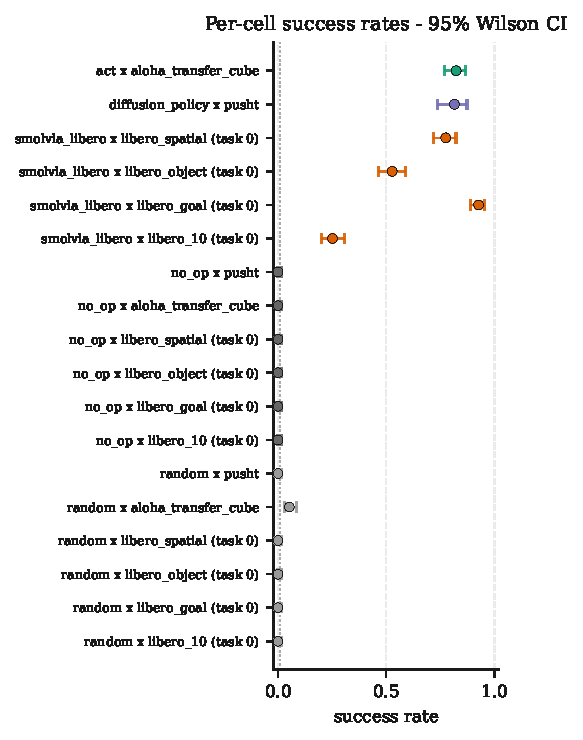
\includegraphics[width=0.6\linewidth]{figures/paper/forest_plot.pdf}
\caption{Per-cell success rate with Wilson 95\% CIs for every v1
leaderboard cell (\S\ref{sec:methods}); the dotted line is the pooled
uniform-random rate. Floor baselines sit at the far left. The four SmolVLA
rows are \emph{task-0-only} cells (\texttt{goal}~$0.928$ down to
\texttt{libero\_10}~$0.252$); the v1.1 suite-averaged rates
(Table~\ref{tab:suite-gap}: $0.813$ down to $0.493$) supersede them as
suite-level statements. \texttt{xvla\_libero} excluded (deferred). Source:
\texttt{results/sweep-full/results.parquet} via
\texttt{src/embodimetry/figures.py:forest\_plot}.}
\label{fig:forest}
\end{figure}

\paragraph{Baseline sanity.}
The floor baselines confirm the bar is real:
no-op succeeds zero times across all six envs ($N{=}1500$, Wilson upper
$0.003$), and uniform-random is above floor only on
\texttt{aloha\_transfer\_cube} ($0.052$~[0.031, 0.087]) --- so the floor
is not one number, which is why we run it on every cell. No floor baseline
was run on the cross-repo Wall env (\S\ref{sec:l3}), an acknowledged gap
in the floor matrix.

\paragraph{Proof the audit bites: a normalization bug we caught in our
own eval.}
A load-bearing result --- evidence the audit machinery
actually catches errors rather than laundering them --- is a bug in
\emph{our own} harness. ACT's apparent failure on
\texttt{aloha\_transfer\_cube} ($\hat{p}{=}0.016$~[0.006, 0.040], below
the env's random floor) turned out to be ours: an early
build of the eval loop silently failed to apply dataset normalization stats
to \texttt{observation.images.top}. PR~\#51 fixed it, and the
same checkpoint reads the canonical \textbf{0.824~[0.772, 0.866]}
(Table~\ref{tab:leaderboard}). A
controlled $2{\times}2$ ablation crossing normalization \{buggy, fixed\}
with inference \{Hub-default, paper-settings\}, each cell $N{=}250$
(Table~\ref{tab:act-ablation}), attributes the recovery to the
normalization fix: broken normalization stays at 0.016 under either
inference setting, while the inference-settings effect within the fixed
row is small and inconclusive ($\Delta\hat{p}{=}0.044$, paired
McNemar $p{=}0.23$), so temporal ensembling
is not the cause of the recovery. Figure~\ref{fig:replication}
plots every cell's measured rate against its paper-reported rate and shows
the $0.016\to0.824$ jump directly. The lesson
generalises: an eval suite must be audited --- normalization,
buffer wiring, observation plumbing --- as carefully as the policies it
scores (Section~\ref{sec:results-audit}). It is not unique to us:
vla-eval~\cite{choi2026vlaeval}, reproducing published VLA scores across
simulation benchmarks, independently documents the same failure class ---
underspecified protocols and undocumented preprocessing that must be
reverse-engineered before published numbers reproduce.

\begin{table}[t]
\centering
\small
\begin{tabular}{lll}
\toprule
& Hub-default inference & Paper-settings inference \\
\midrule
Normalization buggy & 0.016 & 0.016 \\
Normalization fixed & 0.812 & 0.768 \\
\bottomrule
\end{tabular}
\caption{ACT $\times$ \texttt{aloha\_transfer\_cube}, controlled
$2{\times}2$ ablation (normalization $\times$ inference settings), each
cell $N{=}250$ (5~seeds $\times$ 50~episodes). The recovery is
attributable to the
normalization fix (PR~\#51): broken normalization stays at 0.016
regardless of inference settings. Within the fixed row, the
inference-settings comparison shares the seed/episode grid, so it is
paired: $\Delta\hat{p}{=}0.044$ (0.812 vs.\ 0.768), paired-bootstrap 95\%
CI $[-0.020, 0.108]$ crossing zero, McNemar on the discordant pairs
($b{=}40$, $c{=}29$) $p{=}0.23$, Cohen's $h{=}0.108$ --- small and
\emph{inconclusive at this $N$}, below the MDE band
(\S\ref{sec:downscope}); temporal ensembling is therefore not the cause
of the recovery, though a small effect is not ruled out.
The fixed+Hub-default cell (0.812) is the same condition as the
canonical leaderboard number 0.824~[0.772, 0.866] (Table~\ref{tab:leaderboard})
measured in a separate $N{=}250$ run; the two agree within CI. Source:
\texttt{scripts/probes/probe\_act\_normalization\_ablation.py}.}
\label{tab:act-ablation}
\end{table}

\begin{figure}[t]
\centering
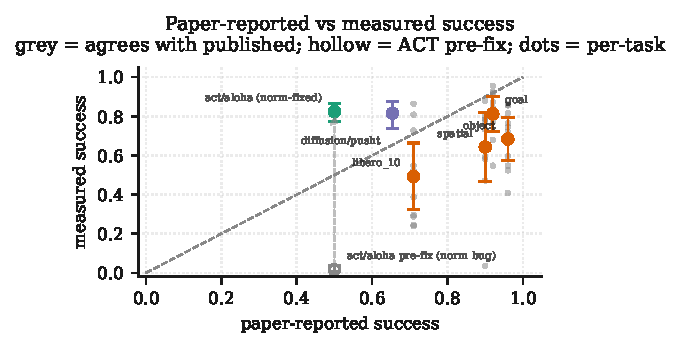
\includegraphics[width=0.62\linewidth]{figures/paper/replication_scatter.pdf}
\caption{Paper-reported vs.\ measured success rate per cell; the $y{=}x$
diagonal is perfect replication. Single-cell ($N{=}250$) points carry
Wilson 95\% error bars and grey out when inside the $N{=}250$ MDE band
($\pm0.123$, ``agrees with paper''); no measured cell qualifies.
ACT~$\times$~\texttt{aloha\_transfer\_cube} plots at its
norm-\emph{fixed} $0.824$, with the pre-fix $0.016$ harness-bug point
(\S\ref{sec:results-audit}) annotated and connected. The four SmolVLA
points (\texttt{spatial}/\texttt{object}/\texttt{goal}/\texttt{libero\_10})
are the v1.1 10-task suite averages of Table~\ref{tab:suite-gap}
($0.643/0.684/0.813/0.493$), with cluster-robust 95\% $t$-CIs over the 10
per-task rates (task as sampling unit, \S\ref{sec:methods}); the small
grey dots behind each mean are those per-task rates --- the within-suite
heterogeneity that rules out episode-iid intervals at suite level.
Source: \texttt{results/sweep-full/results.parquet} (ACT cell spliced to
the corrected rerun) and \texttt{results/sweep-v11-libero/results.parquet},
via \texttt{src/embodimetry/figures.py:replication\_scatter}.}
\label{fig:replication}
\end{figure}

\subsection{The audit pointed outward: SmolVLA's published LIBERO
averages under our protocol}
\label{sec:suite-audit}
The v1 SmolVLA cells were \texttt{task\_id=0} envelopes, so v1 could not
compare against the published 10-task suite
averages~\cite{shukor2025smolvla}. The v1.1 sweep closes that scope gap:
all 10 tasks of all four LIBERO suites, $5$~seeds $\times$ $50$~episodes
per task ($2{,}500$ episodes per suite; $10{,}000$ total, 0 errored),
under the same v1 criterion and checkpoint pin. \textbf{The gap survives
suite-averaging in all four suites}
(Table~\ref{tab:suite-gap}): $-25.7$\,pp (spatial), $-27.6$\,pp (object),
$-10.7$\,pp (goal), $-21.7$\,pp (\texttt{libero\_10}), each rejecting at
$\alpha{=}0.05$ with the task as the sampling unit after Holm correction
(\S\ref{sec:methods}). Object and spatial reject decisively; goal and
\texttt{libero\_10} are solid but not overwhelming (adjusted
$p{=}0.037$ each), and the goal gap is the smallest and must be read as
\emph{statistically marginal}. We frame this as a \emph{protocol-level
discrepancy}, not a ``SmolVLA is worse than reported'' claim: residual
protocol differences remain (seed/trial structure, inherited step caps),
and the published
numbers are $n{=}100$ self-reports whose per-task breakdown is not
released, so a task-paired comparison is not possible.

\begin{table}[t]
\centering
\small
\begin{tabular}{lccccc}
\toprule
Suite & Published ($n{=}100$) & v1.1 suite avg ($n{=}2500$) & Gap &
Cluster-robust 95\% $t$-CI & Holm-adj $p$ \\
\midrule
spatial$^\ddagger$ & 0.90 & 0.643 (1608/2500) & $-25.7$\,pp & [0.466, 0.820] & 0.028 \\
object$^\ddagger$  & 0.96 & 0.684 (1709/2500) & $-27.6$\,pp & [0.572, 0.795] & 0.0013 \\
goal               & 0.92 & 0.813 (2032/2500) & $-10.7$\,pp & [0.724, 0.901] & 0.037 \\
libero\_10         & 0.71 & 0.493 (1232/2500) & $-21.7$\,pp & [0.322, 0.664] & 0.037 \\
\bottomrule
\end{tabular}
\caption{v1.1 suite-averaged SmolVLA rates vs.\ the published suite
averages~\cite{shukor2025smolvla} (10 tasks $\times$ 250 episodes per
suite, equal task weight, matching the paper's equal-task averaging). The
primary test is a one-sample $t$ of the 10 per-task rates against the
published mean (task as sampling unit, Holm-corrected across suites);
Cohen's $h$ on the pooled rates is $0.64/0.79/0.32/0.45$. The goal gap is
the smallest and statistically marginal (adjusted $p{=}0.037$; $p{=}0.026$
re-measured at the canonical 600-step cap), and is never read as decisive.
$^\ddagger$Step-cap caveat travels with spatial/object: their inherited
280-step caps remain unprobed against canonical LIBERO's 600, and the cap
confound is one-directional (a tighter cap can only censor would-be
successes, i.e.\ only widen our measured gap). Source:
\texttt{results/sweep-v11-libero/results.parquet};
\texttt{docs/SWEEP\_V11\_LIBERO\_RESULTS.md}.}
\label{tab:suite-gap}
\end{table}

\paragraph{The cap confound, probed at the canonical cap.}
Every v1.1 failure runs to the step cap --- structurally so, since LIBERO
episodes end only on success or cap, which makes cap-hit rates
uninformative about censoring. The discriminating evidence is the
\emph{success-time tail}: re-running the full goal suite at canonical
cap~600 ($2{,}500$ episodes) leaves the suite average at $0.813$
(2032/2500, the same success count as cap~300; the identity is aggregate,
not episode-level), and only $35/2032$ successes needed more than
300~steps ($1.4$\,pp of episodes; P99 $=374$, max $=567$ of 600). The
directly observed censoring tail bounds the cap effect at
${\lesssim}1.4$\,pp --- an order of magnitude below the $10.7$\,pp goal
gap --- and the gap is now measured \emph{at the canonical cap itself}:
$0.813$ vs.\ published $0.92$, task-level $t$ $p{=}0.026$, cluster-robust
CI $[0.722, 0.904]$ excluding $0.92$. The policy is
\emph{stuck-while-trying}, not slow-but-eventually-correct, replicating
the earlier \texttt{libero\_10} task-0 cap probe ($+0.4$\,pp at cap 600)
at $10\times$ the task coverage. Spatial/object (cap 280) remain the only
unprobed caps, hence the $\ddagger$ in Table~\ref{tab:suite-gap}.

\paragraph{Task heterogeneity, and how representative task 0 was.}
Within-suite per-task rates spread $0.41$--$0.84$ --- the strongest
argument against ever reporting single-task numbers as suite proxies.
Graded against the
suite averages, v1's task-0 envelopes were individually honest but
directionally unrepresentative in \emph{both} directions: task~0
\emph{overstated} the \texttt{libero\_10} gap ($-45.8$\,pp on task~0 vs.\
$-21.7$\,pp suite-level; task 0 is essentially the hardest LIBERO-10
task) and \emph{understated} the spatial/goal gaps (task 0 ranks 2nd of
10 in both) --- precisely the failure mode the v1 claim audit predicted
when it confined those cells to envelope phrasing. The largest
outlier, \texttt{libero\_spatial} task~5 at $0.036$ (9/250), does not
explain the spatial gap: excluding it, the suite average is $0.711$
(1599/2250), still $-18.9$\,pp below published.

\paragraph{Where the failures go: a parquet-joined taxonomy of the
outlier cells.}
A per-episode labeling pass on the five outlier cells (spatial task~5 and
the four hardest \texttt{libero\_10} tasks; $n{=}12$ failures per cell,
selected by a deterministic seed-round-robin rule, labels joined on
\texttt{(policy, env, seed, episode\_index)} against the parquet) shows
the failure mass is \emph{execution}, not time pressure: spatial-t5
fails at the contact-rich ends of an otherwise-complete pick-and-place
routine (place-off-target 7/12, grasp-never-secured 4/12), and the four
\texttt{libero\_10} cells --- all two-object composites --- stall
disproportionately on a small/low-profile second object (pudding box
10/12 in t6, cream-cheese box 8/12 in t7). All 60 labeled failures end at
the cap with the gripper at or hovering over a task-relevant object ---
``stuck-while-trying,'' frame by frame. Counts are observational ($n{=}12$
per cell, no rate claims). Source:
\texttt{docs/assets/failure-taxonomy-labels-v11.csv}.

\paragraph{Internal replication: the v1 cells reproduce a month later.}
The four bare-suite task-0 envs are the same (policy, env, seed-set,
criterion) cells v1 measured in 2026-05; v1.1 re-measured them from
scratch across a month of wall time, harness commits, and sweep restarts.
All four deltas land within $\pm2.4$\,pp with fully overlapping Wilson
CIs (spatial $0.776\to0.800$, object $0.528\to0.524$, goal
$0.928\to0.924$, \texttt{libero\_10} $0.252\to0.244$) --- the strongest
internal-replication evidence the bench has that the eval contract is
stable over time.

\subsection{L3 --- navigation reached, zero contact successes: a
two-endpoint replication}
\label{sec:l3}
This rung is a \emph{strengthened-but-qualified} result (full caveats in
Table~\ref{tab:l3}'s caption). Under matched receding-horizon MPC (re-plan
every step), a zero-training world-model latent-MPC planner reaches
\emph{navigation} while recording zero \emph{contact} successes, in two
independent world-model families --- DINO-WM~\cite{zhou2024dinowm} and
\texttt{facebookresearch/jepa-wms}~\cite{assran2025vjepa2}. On
\textbf{Wall}, two-room point-mass navigation, the planner reaches $4/6$
(JEPA-WM; Wilson 95\% $[0.30, 0.90]$) $\approx 3/6$ (DINO-WM; $[0.19,
0.81]$; the matched seeds-1--6 subset of a fuller 24-episode DINO-WM Wall
run scoring $9/24{=}0.375$, consistent in direction); on \textbf{PushT}, quasi-static contact manipulation, it scores
$0/6$ (JEPA-WM; $[0, 0.39]$) and $0/2$ (DINO-WM; $[0, 0.66]$; this run was
stopped after 2 of 3 requested episodes to stay inside its GPU time box, so
the two families' PushT cells are asymmetric in $N$), moving the block but
pushing it away from the goal --- at a measured ${\approx}35$\,s per
control-step vs.\ ${\approx}0.23$\,s/step (calibrated mean) for the
learned diffusion policy that scores $0.816$ on the same env, a
${\approx}150\times$ per-step compute overhead. We state the evidentiary
status plainly: at these per-cell sample sizes \emph{no per-family
nav-vs-contact contrast is statistically significant on its own} (the
$N{=}6$ Wilson intervals above overlap), and pooling across families would
need its own justification, so the claim rests on the cross-family
\emph{replication of direction} plus the protocol control --- not on any
per-cell test. Two confounds
the earlier reading carried are now controlled: an earlier $0/6$ JEPA-WM
Wall reading came from a full-horizon \emph{one-shot} plan, and matching
the receding-horizon protocol DINO-WM used recovers it to $4/6$, isolating
that $0$ as a planning-protocol artifact rather than a model failure; and
the nav-vs-contact direction no longer rests on one world-model family,
since it replicates across DINO-WM and \texttt{jepa-wms}. The contact
endpoint stays at zero \emph{even with} receding-horizon and in both
families, so the nav$>$contact direction is not a planning-protocol
artifact and not specific to one world-model family. One confound remains
uncontrolled: the two cells still
differ in \emph{env}, and each env requires its own per-env checkpoint, so
env-identity and checkpoint-identity are not separated --- the two-endpoint
design cannot distinguish ``navigation is easier'' from ``this particular
checkpoint is better,'' which is exactly why it is a two-endpoint contrast
and not a controlled sweep.

\begin{table}[t]
\centering
\small
\begin{tabular}{llccc}
\toprule
Env & Dynamics & DINO-WM & JEPA-WM & Per-step compute \\
\midrule
Wall  & 2-room nav (point mass) & $3/6$ [0.19, 0.81] & $4/6$ [0.30, 0.90] & \multirow{2}{*}{${\approx}150\times$ learned policy} \\
PushT & quasi-static contact    & $0/2$ [0.00, 0.66] & $0/6$ [0.00, 0.39] & \\
\bottomrule
\end{tabular}
\caption{The L3 two-endpoint replication (a strengthened-but-qualified
result, \emph{not} a measured curve): the same zero-training latent-MPC
planner under \emph{matched receding-horizon} MPC, run with two independent
world-model families --- DINO-WM~\cite{zhou2024dinowm} and
\texttt{facebookresearch/jepa-wms}~\cite{assran2025vjepa2} --- on a
navigation env (Wall) and a contact env (PushT), on an 8\,GB RTX~4060;
brackets are Wilson 95\% CIs. Both families reach Wall navigation
($4/6 \approx 3/6$); neither records a PushT contact success (JEPA-WM
$0/6$; DINO-WM $0/2$, stopped after 2 of 3 requested episodes inside its
GPU time box --- an $N$-asymmetric cell), so the nav-not-contact
\emph{direction} replicates across families and is not specific to one
world-model family. No per-family contrast is
significant at these $N$; the evidence is the cross-family direction
replication plus the receding-horizon protocol control
(\S\ref{sec:l3}). \textbf{Caveats:} $N{=}6$ episodes per
cell ($N{=}2$ for DINO-WM PushT,
small), and one environment per endpoint, so this is a two-endpoint
contrast and the gradient middle is unmeasured (a MetaWorld middle anchor is
future work). The CEM budget is reduced to fit 8\,GB, below the H100-scale
budgets the source methods use --- a magnitude, not direction, caveat. No
floor baseline was run on Wall (outside the bench's floor matrix).
PushT failures are interpretable --- the planner pushes the block away from
the goal, a contact-modelling failure rather than a bug. Source: cross-repo
\texttt{lerobot-wm-research} (private; available on request, release
planned), run on the same eval contract; not an
in-embodimetry-tree artifact.}
\label{tab:l3}
\end{table}

A $39\times$ predictor speedup (scaled-dot-product attention,
\texttt{bfloat16}, and encode-once frame caching) is what made the L3
loop feasible on this hardware. The misses are interpretable, not bugs:
Wall's are greedy-CEM local minima (wall-trap, last-mile stall) a larger
budget would be expected to escape; PushT's are contact-modelling
failures --- the frozen latent model mispredicts the block's response to
contact, so the planner pushes confidently the wrong way. The explicit
next step is the gradient \emph{middle}: the
same receding-horizon planner on intermediate-dynamics envs (e.g.\ a
MetaWorld reach/multi-contact anchor), so the two endpoints become a swept
curve at a seed count whose Wilson CI clears chance.

\paragraph{Methodology caveats (v1.0.1 audit).}
\label{sec:results-audit}
A static audit surfaced three mismatches that constrain comparative
claims without invalidating any measurement. (1)~\emph{Task scope:} every
v1 SmolVLA cell is \texttt{task\_id=0}, so v1 paper-vs-measured deltas
are single-task envelopes, not replications --- the scope gap the v1.1
10-task sweep closed (\S\ref{sec:suite-audit}). (2)~\emph{ACT
normalization bug} (self-caught, PR~\#51): covered above and in
Table~\ref{tab:act-ablation}. (3)~\emph{LIBERO step caps:} v1 inherited
lerobot caps shorter than canonical LIBERO's
600~\cite{liu2023libero}; the confound has since been probed and bounded
for goal (${\lesssim}1.4$\,pp) and \texttt{libero\_10} task~0
($+0.4$\,pp), and remains open only for spatial/object
(\S\ref{sec:suite-audit}). No patch rewrites a parquet row. Alongside
label-free failure signals (episode-length distributions, plus every
failed-episode MP4) we hand-label failed rollouts into the canonical
six-mode taxonomy: a small curated v1 pass
(\texttt{docs/assets/failure-taxonomy-labels.csv}) and the parquet-joined,
deterministically-sampled v1.1 pass over the outlier cells
(Figure~\ref{fig:failure-taxonomy}; \S\ref{sec:suite-audit}). XVLA ran on
LIBERO but is deferred from v1
over an unresolved Hub-artifact wiring bug
(\texttt{docs/DEFERRED\_POLICIES.md}).

\begin{figure}[t]
  \centering
  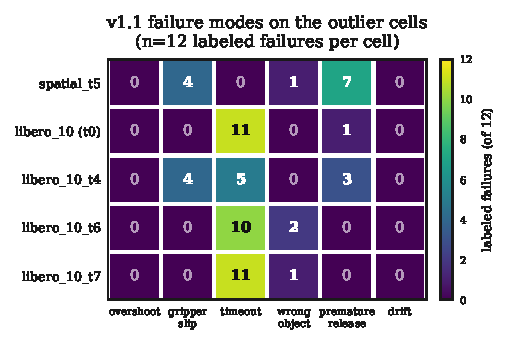
\includegraphics[width=0.62\linewidth]{figures/paper/failure_taxonomy_v11.pdf}
  \caption{The v1.1 failure taxonomy on the five outlier cells
  (\texttt{spatial\_t5} and the four hardest \texttt{libero\_10} tasks):
  counts of hand-labeled failed episodes per canonical mode
  (\S\ref{sec:methods}; \texttt{docs/FAILURE\_TAXONOMY.md}), $n{=}12$
  failures per cell, deterministic seed-round-robin sampling, labels
  joined on \texttt{(policy, env, seed, episode\_index)} against the
  per-episode parquet. Modes with zero labeled episodes are shown as
  explicit zero cells rather than dropped. Counts are observational: at
  $n{=}12$ per cell no within- or cross-cell rate claim is supported ---
  the cross-cell reading (execution failure at contact-rich ends, stalls
  on small second objects) is \S\ref{sec:suite-audit}'s. Single labeler,
  no agreement statistic, same caveat as the v1 pass. Source:
  \texttt{docs/assets/failure-taxonomy-labels-v11.csv} via
  \texttt{src/embodimetry/figures.py:failure\_taxonomy\_v11}.}
  \label{fig:failure-taxonomy}
\end{figure}

% ---------------------------------------------------------------- %
% Discussion                                                       %
% ---------------------------------------------------------------- %

\section{Discussion}

\paragraph{What the ladder says.}
Three things stand: the cross-paradigm contract and the self-auditing
methodology are settled, citable contributions; the L3 reading is the
strengthened-but-qualified result the contract was purpose-built to
produce (\S\ref{sec:l3}). The self-audit claim is narrow and defensible: a
neutral seed/Wilson-CI/MDE contract surfaced a normalization bug that
pinned ACT$\times$aloha at $0.016$ (below the random floor), a clean
$2{\times}2$ ablation attributed the recovery to the
fix (Table~\ref{tab:act-ablation}) --- an error a loss curve hides and only
a closed-loop CI exposes --- and a guard test (\S\ref{sec:guard})
code-enforces that the rung above keeps its caveats. Pointed outward, the
same machinery turned v1's single-task envelopes into the four-suite
protocol-level discrepancy of \S\ref{sec:suite-audit} --- and graded its
own v1 claims against the fuller measurement, validating the envelope
caveats it had pre-registered. The instrument is also demonstrably
stable: the four v1 LIBERO cells re-measured from scratch a month later
reproduce within $\pm2.4$\,pp with fully overlapping CIs
(\S\ref{sec:suite-audit}). The supporting spine
is the set of honest negatives of \S\ref{sec:results} --- an inconclusive
fine-tune and a collapsed LoRA track (neither inflated into a win), and a
classical controller whose ${\sim}1\%$ strict rate against
${\sim}50\%$ mean coverage locates the value of learning in the last
fraction of precision.
The two contributions we stand behind without qualification are
the \emph{contract} and the \emph{self-audit}; the third, the L3
two-endpoint nav-vs-contact replication, stays qualified exactly as
\S\ref{sec:l3} states it.

\subsection{Why the two endpoints behave differently, and what would
turn them into a curve}
Wall's point-mass dynamics are low-dimensional, near-linear, and
contact-free, so a frozen latent forward model predicts them accurately
enough that receding-horizon CEM finds a goal-reaching plan it was never
trained on --- for \emph{both} world-model families, so the reading is
\emph{consistent with} a property of the dynamics rather than of one
checkpoint (the env/checkpoint confound of \S\ref{sec:l3} is not ruled
out; family replication rules out family-specificity only). PushT's
contact-rich, stiff dynamics compound small latent errors through
contact --- in both families. So ``do we need a learned policy?''
already looks, at the two
endpoints, like a question about the modellability of the dynamics. What
would turn the two endpoints into a measured curve is the study the
contract enables: the \emph{same} receding-horizon planner at the
\emph{same} budget across a \emph{sequence} of envs (point-nav $\to$ reach
$\to$ contact $\to$ deformable, with a MetaWorld middle anchor), each at a
seed count whose Wilson CI clears chance, with the planner's compute cost
(measured at ${\approx}150\times$ per step here) reported alongside.

\subsection{Limitations}

\begin{itemize}\setlength{\itemsep}{0pt}\setlength{\parskip}{0pt}\setlength{\topsep}{0pt}\setlength{\partopsep}{0pt}
    \item \textbf{Simulation only.} All numbers are sim; the sim-to-real
    gap is unmeasured. embodimetry is a screening tool, not a
    substitute for hardware evaluation.
    \item \textbf{Single-hardware wall-clock.} Per-step latency is from
    one RTX~4060 laptop; absolute ms/step differs across GPUs, but the
    \emph{ranking} the auto-downscope rule consumes is portable.
    \item \textbf{$\boldsymbol{\pi_0}$ family deferred.} $\pi_0$,
    $\pi_0$-FAST, $\pi_{0.5}$ need ${\approx}30$\,GB host
    RAM at \texttt{from\_pretrained} cold load,
    exceeding the 32\,GB v1 laptop's headroom; v1 compares four learned
    policies, not seven.
    \item \textbf{L3 is a strengthened two-endpoint result, not a curve and
    not a cross-env law} (\S\ref{sec:l3}): $N{=}6$ episodes per cell
    ($N{=}2$ for DINO-WM PushT; no per-family
    contrast significant on its own), one environment per
    endpoint, so
    the gradient \emph{middle} (reach, multi-contact, deformable) is
    unmeasured and a MetaWorld middle anchor is future work. The CEM budget
    is reduced to fit 8\,GB (a magnitude, not direction, caveat) and the
    cells are a
    \emph{cross-repo} artifact (\texttt{lerobot-wm-research}, private:
    available on request, release planned), not an
    in-tree parquet of this repository.
    \item \textbf{Single-GPU compute ceiling.} Everything runs on
    one 8\,GB RTX~4060 laptop: SmolVLA
    full fine-tune does not fit, so L1 is a single ACT cell plus the
    collapsed SmolVLA LoRA track ($0.252\to0/50$ on a
    seed-0 probe; $0/100$ pooled),
    reported as a failed lift rather than dropped.
    \item \textbf{L1 is one cell, and the lift is inconclusive.} The
    fine-tuning rung is ACT$\times$aloha alone; its $+0.040$ shift has an
    unpaired 95\% CI of $[-0.024, 0.104]$ and $h{=}0.11$ (below the
    $N{=}250$ MDE), and the per-episode fine-tuned outcomes were not
    retained, so the promised paired test could not be computed. We
    cannot claim fine-tuning helps \emph{or} that it does nothing from
    this cell; a
    multi-cell L1 sweep with a larger demo budget and a from-scratch
    baseline is needed to say anything stronger.
    \item \textbf{Residual protocol differences in the suite comparison.}
    The four-suite gap (\S\ref{sec:suite-audit}) is a protocol-level
    discrepancy, not a model claim: our 5~seeds $\times$ 50~episodes
    vs.\ the paper's~\cite{shukor2025smolvla} 10~trials per task
    (initial-state distributions may differ), spatial/object step caps
    unprobed against canonical 600 (one-directional confound: can only
    widen our gap), and $n{=}100$ published self-reports with no per-task
    breakdown, so no task-paired test is possible.
    \item \textbf{Sparse matrix, multi-comparison, and episode budget.}
    Cross-policy comparisons are valid only within shared envs; the
    L0/L1/L2 rungs sit on \emph{different} envs (PushT, aloha), so they are
    same-contract but not same-task and must be read as paradigm snapshots,
    not a head-to-head. With several pairwise claims in play we control
    family-wise error by Holm--Bonferroni, but the matrix is too sparse for
    a fully crossed comparison. $N{=}250$ is a GPU-budget choice; claims
    cite only deltas above the per-cell MDE.
    \item \textbf{Harness bugs and protocol-vs-paper.} Our own
    normalization bug (PR~\#51) shows a harness can be the dominant error
    source; the LIBERO cap mismatches make those cells protocol-vs-paper,
    not replication failures. Cross-policy paired tests defer to a future
    release when XVLA returns.
\end{itemize}

\paragraph{Future work.}
Turn the two L3 endpoints into a measured curve: the \emph{same}
receding-horizon planner, a larger seed count and paper-faithful CEM
budget, varying \emph{only} the env across the gradient middle (point-nav
$\to$ reach $\to$ contact $\to$ deformable, with a MetaWorld anchor), at a
seed count whose Wilson CIs clear chance. Broaden L1 to a multi-cell,
larger-budget fine-tuning sweep with a from-scratch baseline so the rung
can support a positive claim, and diagnose the SmolVLA LoRA collapse.
Close the last open cap caveat (a canonical-cap probe for
spatial/object, cap 280); onboard the $\pi_0$
family via quantized/streaming load; and re-run on hardware for the
sim-to-real gap.

\section{Conclusion}
embodimetry puts four robot-control paradigms on one seed/CI/MDE
contract and then holds the contract to its own standard. The instrument
caught its own normalization bug and attributed the $0.016\to0.824$
recovery with a controlled ablation; pointed outward, it measured a
four-suite protocol-level discrepancy against published LIBERO numbers
that survives suite averaging under cluster-robust tests; and it kept
every negative --- an inconclusive fine-tune, a collapsed LoRA track, a
${\sim}1\%$ classical controller, and a world-model planner with zero
contact successes --- on the board with its evidence attached. The
contract, the code-enforced self-audit, and the qualified two-endpoint
world-model reading are the contributions; everything else is a caveat we
measured, bounded, or explicitly left open.

% ---------------------------------------------------------------- %
% References                                                       %
% ---------------------------------------------------------------- %

\begin{multicols}{3}
{\scriptsize
\setlength{\itemsep}{0pt}
\bibliographystyle{plain}
\bibliography{references}
}
\end{multicols}

\end{document}
